% !TEX TS-program = pdflatex
% !TEX encoding = UTF-8 Unicode

% This is a simple template for a LaTeX document using the "article" class.
% See "book", "report", "letter" for other types of document.

\documentclass[11pt]{article} % use larger type; default would be 10pt

%%% Examples of Article customizations
% These packages are optional, depending whether you want the features they provide.
% See the LaTeX Companion or other references for full information.
\counterwithin{figure}{section}
%%% PAGE DIMENSIONS
\usepackage{geometry} % to change the page dimensions
\geometry{a4paper} % or letterpaper (US) or a5paper or....
% \geometry{margin=2in} % for example, change the margins to 2 inches all round
% \geometry{landscape} % set up the page for landscape
%   read geometry.pdf for detailed page layout information
\usepackage[]{svg}

\usepackage{pdfpages}

\usepackage{graphicx,tikz} % support the \includegraphics command and options
\usepackage{tikz-cd}
\usepackage{relsize,nicematrix}
\usetikzlibrary{matrix, calc, arrows}
\usepackage{tikz-dimline}
\usetikzlibrary{patterns,positioning}
\usepackage{listings,svg,fancyhdr}

% \usepackage[parfill]{parskip} % Activate to begin paragraphs with an empty line rather than an indent

%%% PACKAGES
\usepackage{booktabs,amsmath,mathtools} % for much better looking tables
\usepackage{array} % for better arrays (eg matrices) in maths
\usepackage{paralist} % very flexible & customisable lists (eg. enumerate/itemize, etc.)
\usepackage{verbatim} % adds environment for commenting out blocks of text & for better verbatim


\usepackage[pagebackref=true, colorlinks, linkcolor=blue, citecolor=magenta, urlcolor=cyan] {hyperref}%


%\usepackage{sansmath}
%\sansmath
%\usepackage{palatino}

\usepackage{cleveref,booktabs,multirow} % make it possible to include more than one captioned figure/table in a single float
% These packages are all incorporated in the memoir class to one degree or another...

\usepackage{tcolorbox}


\usepackage{matlab-prettifier}
\usepackage{pythonhighlight}

%%% HEADERS & FOOTERS
\usepackage{fancyhdr,caption,subcaption} % This should be set AFTER setting up the page geometry
\pagestyle{fancy} % options: empty , plain , fancy
\renewcommand{\headrulewidth}{0pt} % customise the layout...
\lhead{}\chead{}\rhead{}
\lfoot{}\cfoot{\thepage}\rfoot{}
\usepackage{pgfplots,relsize}
%%% SECTION TITLE APPEARANCE
%\usepackage{sectsty}
%\allsectionsfont{\sffamily\mdseries\upshape} % (See the fntguide.pdf for font help)
% (This matches ConTeXt defaults)

%%% ToC (table of contents) APPEARANCE
\usepackage[nottoc,notlof,notlot]{tocbibind} % Put the bibliography in the ToC
\usepackage[titles,subfigure]{tocloft} % Alter the style of the Table of Contents
\renewcommand{\cftsecfont}{\rmfamily\mdseries\upshape}
\renewcommand{\cftsecpagefont}{\rmfamily\mdseries\upshape} % No bold!


\newcommand{\matindex}[1]{\mbox{\scriptsize#1}}
\crefname{section}{\S}{\S\S}

%%% The "real" document content comes below...
% Define a custom color
\definecolor{backcolour}{rgb}{0.95,0.95,0.92}
\definecolor{codegreen}{rgb}{0,0.6,0}

%\usepackage[symbol]{footmisc}
%
%\renewcommand{\thefootnote}{\fnsymbol{footnote}}
%\footnote[num]{text}
\renewcommand*{\thefootnote}{\fnsymbol{footnote}}
\newcommand\pcref[1]{(\cref{#1})}
% Define a custom style
\lstdefinestyle{myStyle1}{
    backgroundcolor=\color{backcolour},   
    commentstyle=\color{codegreen},
    basicstyle=\ttfamily\footnotesize,
    breakatwhitespace=false,         
    breaklines=true,                 
    keepspaces=true,                 
    numbers=left,       
    numbersep=5pt,                  
    showspaces=false,                
    showstringspaces=false,
    showtabs=false,                  
    tabsize=2,
}

% Use \lstset to make myStyle the global default

\lstdefinestyle{myStyle2}{
    belowcaptionskip=1\baselineskip,
    breaklines=true,
    frame=none,
    numbers=none,
    basicstyle=\footnotesize\ttfamily,
    keywordstyle=\bfseries\color{green!40!black},
    commentstyle=\itshape\color{purple!40!black},
    identifierstyle=\color{blue},
    backgroundcolor=\color{gray!10!white},
}


\title{Thick cylinder under pressure}
\author{Mohammad Abazari}
\date{July 28, 2022}
\begin{document}
\maketitle
\tableofcontents
\section{Lame's problem-Thick cylinder subjected to internal pressure}\label{sec_theory}
Consider a thick cylinder of inner radius $R_i$, outer radius $R_o$, length $L$ subjected to internal pressure $P_i$ and outer pressure $P_o=0$. Two cases of plane-stress $\sigma_z=0$ and -strain $\varepsilon_z=0$ are studied.
\subsection{Plane stress}
Assuming that both cylinder ends are free thus $\sigma_z=0$,
\begin{equation}\nonumber
\frac{\partial\sigma_r}{\partial r}+\frac{\sigma_r-\sigma_\theta}{r}=0
\end{equation}
$r$ is the only independent variable in this expression which could be rewriten as below
\begin{equation}\label{eq1}
\frac{\mathrm{d}}{\mathrm{d}r}(r\sigma_r)-\sigma_\theta=0
\end{equation}
Following Hooke's law\cite{hooke1678},
\begin{equation}\nonumber\begin{aligned}
\varepsilon_r =& \frac{1}{E}\left(\sigma_r-\nu\sigma_\theta\right)\\
\varepsilon_\theta =& \frac{1}{E}\left(\sigma_r-\nu\sigma_\theta\right)\\
\sigma_r =& \frac{E}{1-\nu^2}\left(\varepsilon_r+\nu\varepsilon_\theta\right)\\
\sigma_\theta =& \frac{E}{1-\nu^2}\left(\varepsilon_\theta-\nu\varepsilon_r\right)
\end{aligned}
\end{equation}
Substituting strain equations,
\begin{equation}\label{eq2}\begin{aligned}
\sigma_r =& \frac{E}{1-\nu^2}\left(\frac{\mathrm{d}u_r}{\mathrm{d}r}+\nu\frac{u_r}{r}\right)\\
\sigma_\theta =& \frac{E}{1-\nu^2}\left(\frac{u_r}{r}+\nu\frac{\mathrm{d}u_r}{\mathrm{d}r}\right)
\end{aligned}
\end{equation}
Substituting the above in \cref{eq1}
\begin{equation}\nonumber
\begin{aligned}
\frac{\mathrm{d}}{\mathrm{d}r}\left(r\frac{\mathrm{d}u_r}{\mathrm{d}r}+vu_r\right)-\left(\frac{u_r}{r}+v\frac{\mathrm{d}u_r}{\mathrm{d}r}\right)=&0\\
\frac{\mathrm{d}u_r}{\mathrm{d}r}+r\frac{\mathrm{d}^2u_r}{\mathrm{d}r^2}+\nu\frac{\mathrm{d}u_r}{\mathrm{d}r}-\frac{u_r}{r}-\nu\frac{\mathrm{d}u_r}{\mathrm{d}r}=&0\\
\frac{\mathrm{d}^2u_r}{\mathrm{d}r^2}+\frac{1}{r}\frac{\mathrm{d}u_r}{\mathrm{d}r}-\frac{u_r}{r^2}=&0\\
\frac{\mathrm{d}}{\mathrm{d}r}\left[\frac{1}{r}\frac{\mathrm{d}}{\mathrm{d}r}(u,r)\right]=&0
\end{aligned}
\end{equation}
Assuming $u_r$ follows the below function
\begin{equation}\label{eqs03}
u_r=C_1r+\frac{C_2}{r}
\end{equation}
Substituting the above in \cref{eq2},
\begin{equation}\begin{aligned}
\sigma_r =& \frac{E}{1-\nu^2}\left[C_1(1+\nu)-C_2(1-\nu)\frac{1}{r^2}\right]\\
\sigma_\theta =& \frac{E}{1-\nu^2}\left[C_1(1+\nu)+C_2(1-\nu)\frac{1}{r^2}\right]
\end{aligned}
\end{equation}
\begin{figure}\centering
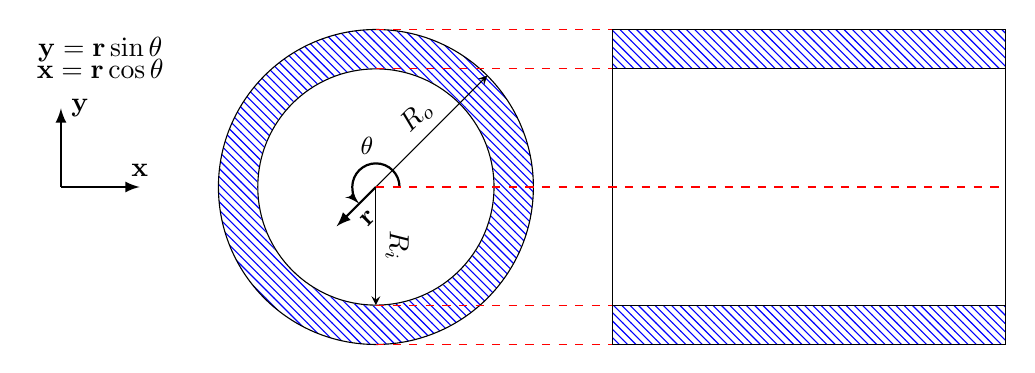
\begin{tikzpicture}
\draw [fill,black,pattern=north west lines, pattern color=blue](0,0) circle(2);
\draw [fill,white](0,0) circle(1.5);\draw [black](0,0) circle(1.5);
\draw [->,>=stealth] (0,0)--(0,-1.5) node[midway,above,sloped]{$R_i$};
\draw [->,>=stealth] (0,0)--(1.4142,1.4142)node[midway,above,sloped]{$R_o$};
\draw [->,>=latex,thick] (0,0)--(-0.5,-0.5)node[midway,below,sloped]{$\mathbf{r}$};
\draw[->,>=latex',thick] (0.3,0) arc[radius=0.3, start angle=0, end angle=225] node[midway,above] {\small$\mathbf{\theta}$};
\draw [fill,black,pattern=north west lines, pattern color=blue](3,-2) rectangle (8,2);
\draw [black,fill,white](3,-1.5) rectangle (8,1.5);
\draw [black](3,-1.5) rectangle (8,1.5);

\draw [dashed,red] (0,0)--(8,0);
\draw [dashed,red] (0,2)--(3,2);
\draw [dashed,red] (0,-2)--(3,-2);
\draw [dashed,red] (0,-1.5)--(3,-1.5);
\draw [dashed,red] (0,1.5)--(3,1.5);

\draw [thick,->,>=latex] (-4,0) -- (-3,0) node[above]{$\mathbf{x}$};
\draw [thick,->,>=latex] (-4,0) -- (-4,1) node[right]{$\mathbf{y}$};
\draw [](-3.5,1.5) node[]{$\mathbf{x}=\mathbf{r}\cos\mathbf{\theta}$};
\draw [](-3.5,1.75) node[]{$\mathbf{y}=\mathbf{r}\sin\mathbf{\theta}$};

\end{tikzpicture}
\caption{Problem geometry.}\label{fig01geom}
\end{figure}
Constants $C_1$ and $C_2$ are applying boundary conditions.
\begin{equation}\nonumber
\begin{aligned}
\sigma_r(r=R_i) = &-P_i= \frac{E}{1-\nu^2}\left[C_1(1+\nu)-C_2(1-\nu)\frac{1}{R_i^2}\right]\\
\sigma_r(r=R_o) = &-P_o=0=\frac{E}{1-\nu^2}\left[C_1(1+\nu)-C_2(1-\nu)\frac{1}{R_o^2}\right]\\
\end{aligned}
\end{equation}
Solving for these two constants,
\begin{equation}\nonumber
\begin{aligned}
C_1=&\frac{1-\nu}{E}\frac{P_iR_i^2-P_oR_o^2}{R_o^2-R_i^2}\\
C_2=&\frac{1+\nu}{E}\frac{R_i^2-R_o^2}{R_o^2-R_i^2}\left(P_i-P_o\right)
\end{aligned}
\end{equation}
Substituting these constants into the above equations
\begin{equation}\label{eqs04}
\begin{aligned}
\sigma_{r}=&\frac{P_i R_i^{2}-P_o R_o^{2}}{R_o^{2}-R_i^{2}}-\frac{R_i^{2} R_o^{2}}{r^{2}} \frac{P_i-P_o}{R_o^{2}-R_i^{2}}\\
\sigma_{\theta}=&\frac{P_i R_i^{2}-P_o R_o^{2}}{R_o^{2}-R_i^{2}}+\frac{R_i^{2} R_o^{2}}{r^{2}} \frac{P_i-P_o}{R_o^{2}-R_i^{2}}
\end{aligned}
\end{equation}
\subsubsection{Plane stress problem with internal pressure}
If outside pressure
$P_o=0$,
then
%\begin{equation}\nonumber
\begin{align}
\sigma_{r}=&\frac{P_i R_i^{2}}{R_o^{2}-R_i^{2}}\left[1-\frac{R_o^2}{r^2}\right]\label{eqs01}\\
\sigma_{\theta}=&\frac{P_i R_i^{2}}{R_o^{2}-R_i^{2}}\left[1+\frac{R_o^2}{r^2}\right]\label{eqs02}\\
\end{align}
%\end{equation}
The above derivation shows that $\sigma_r$ is compressive through the cylinder thickness while and $\sigma_\theta$ is tensile and positive.
\begin{figure}\centering
\begin{subfigure}{0.45\textwidth}
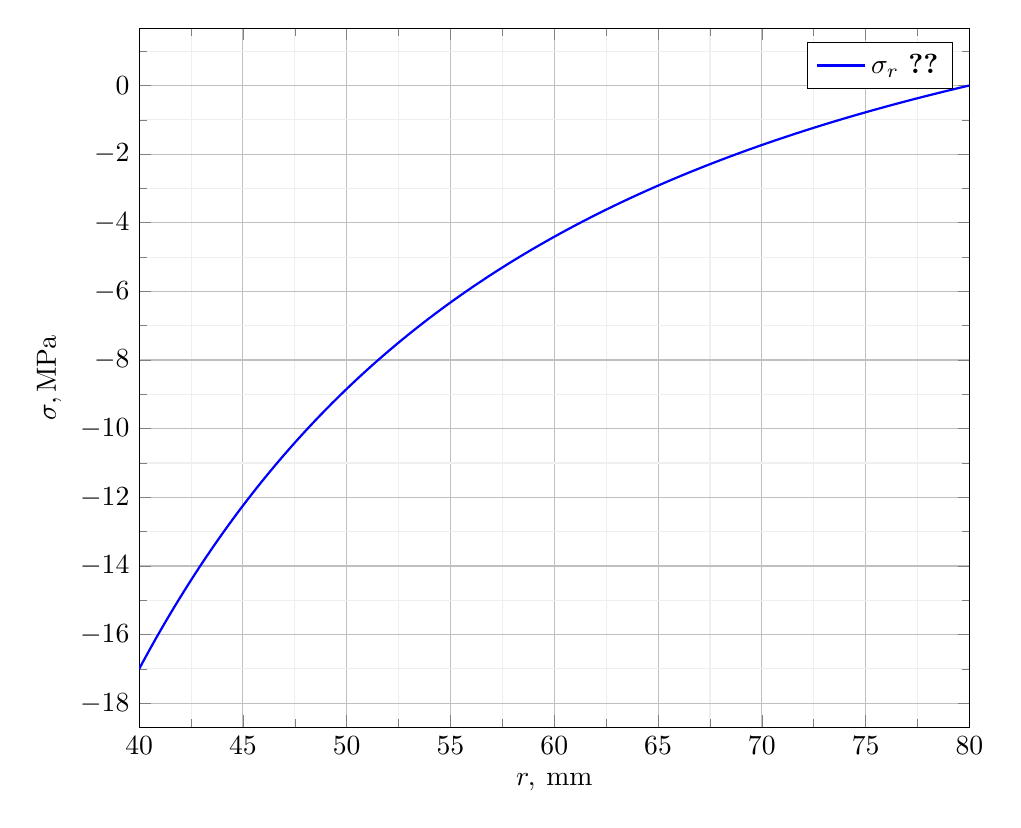
\begin{tikzpicture}
\begin{axis}[
	xmin = 40, xmax = 80,
%	xtick distance = 2.5,
%	ytick distance = 0.5,
	grid = both,
	minor tick num = 1,
	major grid style = {lightgray},
	minor grid style = {lightgray!25},
	width = \textwidth,
	ylabel = {$\sigma,\mathrm{MPa}$},
	xlabel = {$r,\:\mathrm{mm}$},
%	height = 0.5\textwidth,
]
	\addplot[
		domain = 40:80,
		samples = 200,
		smooth,
		thick,
		blue,
	] {17*40^2/(80^2-40^2)*(1-80^2/x^2)};
	\addlegendentry{{$\sigma_r$ \cref{eqs01}}}
\end{axis}
\end{tikzpicture}\end{subfigure}\:\:\:\:\:\:\:\:\begin{subfigure}{0.45\textwidth}
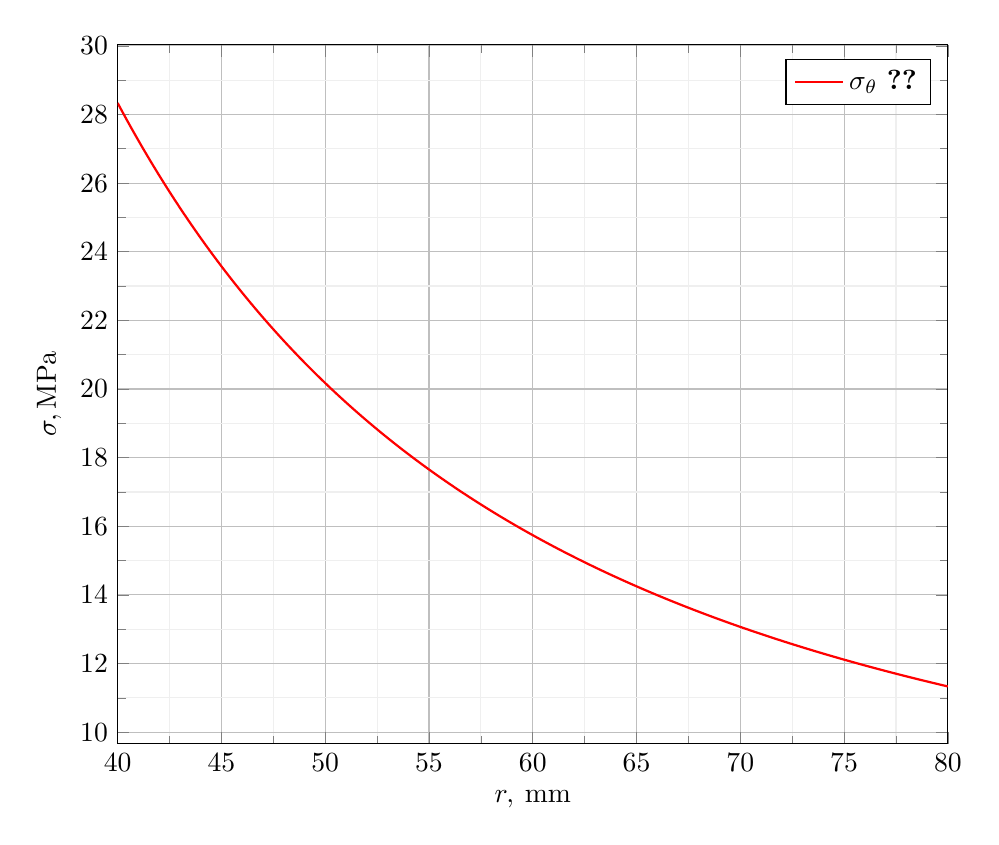
\begin{tikzpicture}
\begin{axis}[
	xmin = 40, xmax = 80,
%	xtick distance = 2.5,
%	ytick distance = 0.5,
	grid = both,
	minor tick num = 1,
	major grid style = {lightgray},
	minor grid style = {lightgray!25},
	width = \textwidth,
	ylabel = {$\sigma,\mathrm{MPa}$},
	xlabel = {$r,\:\mathrm{mm}$},
%	height = 0.5\textwidth,
]
	\addplot[
		domain = 40:80,
		samples = 200,
		smooth,
		thick,
		red,
	]{17*40^2/(80^2-40^2)*(1+80^2/x^2)};
	\addlegendentry{{$\sigma_\theta$ \cref{eqs02}}}
\end{axis}
\end{tikzpicture}\end{subfigure}
\end{figure}
\subsection{Plane strain}
In the plane strain case, $\sigma_z$ is assumed constant, \cref{eq1}
\begin{equation}\nonumber
\frac{\mathrm{d}}{\mathrm{d}r}(r\sigma_r)-\sigma_\theta=0
\end{equation}
From Hooke's law\cite{hooke1678}
\begin{equation}\nonumber
\begin{aligned}
\varepsilon_{r}=&\frac{1}{E}\left[\sigma_{r}-v\left(\sigma_{\theta}+\sigma_{z}\right)\right]\\
\varepsilon_{\theta}=&\frac{1}{E}\left[\sigma_{\theta}-v\left(\sigma_{r}+\sigma_{z}\right)\right]\\
\varepsilon_{z}=&\frac{1}{E}\left[\sigma_{r}-v\left(\sigma_{r}+\sigma_{\theta}\right)\right]
\end{aligned}
\end{equation}
With
 $\varepsilon_z=0$
\begin{equation}\nonumber
\begin{aligned}
\sigma_{z}=&v\left(\sigma_{r}+\sigma_{\theta}\right)\\
\varepsilon_{r}=&\frac{1+v}{E}\left[(1-v) \sigma_{r}-v \sigma_{\theta}\right]\\
\varepsilon_{\theta}=&\frac{1+v}{E}\left[(1-v) \sigma_{\theta}-v \sigma_{r}\right]
\end{aligned}
\end{equation}
Solving for stress components
\begin{equation}\nonumber
\begin{aligned}
\sigma_{\theta}=&\frac{E}{(1-2 v)(1+v)}\left[v \varepsilon_{r}+(1-v) \varepsilon_{\theta}\right]\\
\sigma_{r}=&\frac{E}{(1-2 v)(1+v)}\left[(1-v) \varepsilon_{r}+v \varepsilon_{\theta}\right]
\end{aligned}\end{equation}
Substituting strain
\begin{equation}\label{eq4}
\begin{aligned}
\sigma_{r}=&\frac{E}{(1-2 v)(1+v)}\left[(1-v) \frac{d u_{r}}{d r}+v \frac{u_{r}}{r}\right]\\
\sigma_{\theta}=&\frac{E}{(1-2 v)(1+v)}\left[v \frac{d u_{r}}{d r}+(1-v) \frac{u_{r}}{r}\right]\\
\end{aligned}
\end{equation}
Substituting the above in the equilibrum equations
\begin{equation}\nonumber\begin{aligned}
\frac{\mathrm{d}}{\mathrm{d} r}\left[(1-v) r \frac{d u_{r}}{d r}+v u_{r}\right]-v \frac{d u_{r}}{d r}-(1-v) \frac{u_{r}}{r}&=0\\
\frac{d u_{r}}{d r}+r \frac{\mathrm{d}^{2} u_{r}}{\mathrm{d} r^{2}}-\frac{u_{r}}{r}&=0\\
\frac{\mathrm{d}}{\mathrm{d} r}\left(\frac{\mathrm{d} u}{\mathrm{d} r}+\frac{u_{r}}{r}\right)&=0
\end{aligned}
\end{equation}
Assuming \cref{eqs03} for $u_r$ and substituting into \cref{eq4}
\begin{equation}\nonumber\begin{aligned}
\sigma_{\theta}=&\frac{E}{(1-2 v)(1+v)}\left[C_{1}+(1-2 v) \frac{C_{2}}{r^{2}}\right]\\
\sigma_{r}=&\frac{E}{(1-2 v)(1+v)}\left[C_{1}-(1-2 v) \frac{C_{2}}{r^{2}}\right]
\end{aligned}
\end{equation}
Again applying boundary conditions
\begin{equation}\nonumber
\begin{aligned}
\sigma_r(r=R_i)=&-P_i=\frac{E}{(1-2 v)(1+v)}\left[C_{1}-(1-2 v) \frac{C_{2}}{R_i^{2}}\right]\\
\sigma_r(r=R_o)=&-P_{o}=\frac{E}{(1-2 v)(1+v)}\left[C_{1}+(1-2 v) \frac{C_{2}}{R_o^{2}}\right]
\end{aligned}
\end{equation}
Thus,
\begin{equation}\nonumber\begin{aligned}
C_{1}=&\frac{(1-2 v)(1+v)}{E} \frac{P_{o} R_o^{2}-P_{i} R_i^{2}}{R_i^{2}-R_o^{2}}\\
C_{2}=&\frac{1+v}{E} \frac{\left(P_{o}-P_{i}\right) R_i^{2} R_o^{2}}{R_i^{2}-R_o^{2}}
\end{aligned}
\end{equation}
Substituting these constants into the above,
\begin{equation}\nonumber\begin{aligned}
\sigma_{r}=&\frac{P_{i} R_i^{2}-P_{o} R_o^{2}}{R_o^{2}-R_i^{2}}-\frac{R_i^{2} R_o^{2}}{r^{2}} \frac{P_{i}-P_{o}}{R_o^{2}-R_i^{2}} \\
\sigma_{\theta}=&\frac{P_{i} R_i^{2}-P_{o} R_o^{2}}{R_o^{2}-R_i^{2}}+\frac{R_i^{2} R_o^{2}}{r^{2}} \frac{P_{i}-P_{o}}{R_o^{2}-R_i^{2}}
\end{aligned}
\end{equation}
Which equals \cref{eqs04}.
\section{MATLAB modeling}\label{sec_numm}
A cylinder of inner radius of
$R_i=40\mathrm{mm}$
outer radius
 $R_o=80\mathrm{mm}$
length 
  $L=1000\mathrm{mm}$
inside pressure
   $17\mathrm{MPa}$
outside pressure
    $2$
was meshed with minimum element dimension of 
     $1\mathrm{mm}$
      and maximum element dimension of
      $10\mathrm{mm}$.
\begin{figure}\centering
\includegraphics[width=0.4\textwidth]{Figures/fig01.pdf}
\caption{3D model geometry.}\label{fig01}
\end{figure}
\begin{figure}\centering
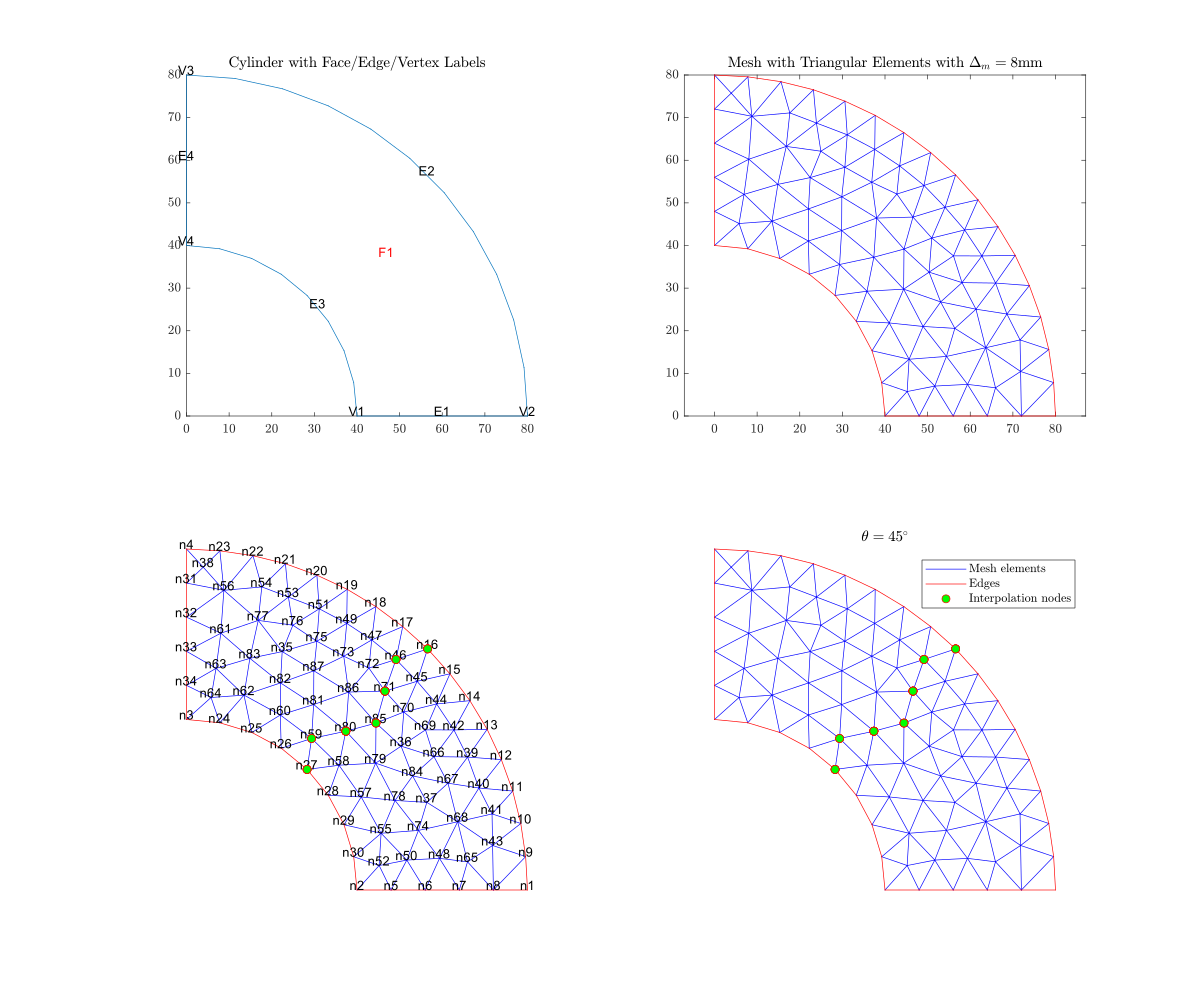
\includegraphics[width=\textwidth, trim={3cm 3cm 1cm 1cm},clip]{Figures/fig01m8.pdf}
\caption{2D model and mesh.}\label{fig01m}
\end{figure}

\begin{figure}\centering
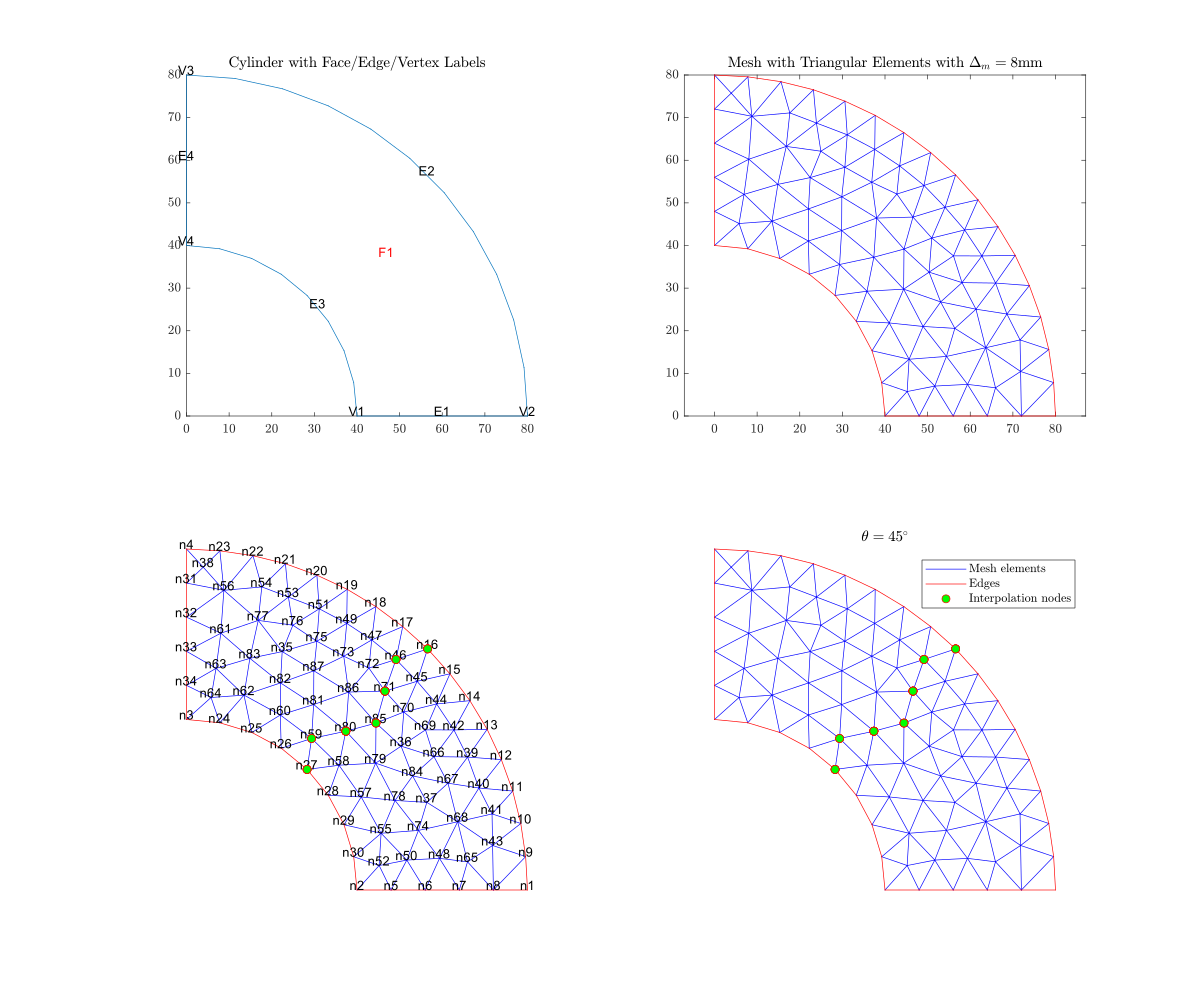
\includegraphics[width=\textwidth, trim={3cm 3cm 1cm 1cm},clip]{Figures/fig01m8.pdf}
\caption{3D model and mesh.}\label{fig01m}
\end{figure}

\begin{figure}\centering
\begin{subfigure}{\textwidth}\centering
\includegraphics[width=0.8\textwidth,trim={1cm 1cm 1cm 0cm},clip]{Figures/fig03m8.pdf}
\caption{2D results.}\label{fig05a}
\end{subfigure}
\begin{subfigure}{\textwidth}\centering
%\input{Figures/fig05}
\includegraphics[width=0.8\textwidth,trim={1cm 1cm 1cm 0cm},clip]{Figures/fig05m10.pdf}
\caption{3D results, $\Delta.$}\label{fig05b}
\end{subfigure}
\caption{Radial variation of stress components.}\label{fig05}
\end{figure}

\begin{figure}\centering
%\input{Figures/fig06}
\includegraphics[width=0.8\textwidth,trim={1cm 1cm 1cm 0cm},clip]{Figures/fig06m10.pdf}
\caption{Stress variation in length.}\label{fig06}
\end{figure}
\section{Conclusions}
\begin{itemize} 
\item Both 2D and 3D numerical models \pcref{sec_numm} agree with theoretical derivation \pcref{sec_theory} \pcref{fig05}.
\item Based on both numerical and theoretical results radial ($\sigma_r$) and angular stresses ($\sigma_\theta$) reduce radially\pcref{fig05}.
\item 3D numerical results shows no significant change in longitudinal stress ($\sigma_z$) which sattisfies the plane stress and strain assumptions\pcref{fig06}.
\item Longitudinal stress oscilations in the cylinder length \pcref{fig06} showcases model sensitivity to proper boundary conditions which is dealt with through finer mesh sizes.
\end{itemize}
\newpage
\section{Appendices}\subsection{Stress transformation from cartesian to cylindrical coordinates}
\includepdf[pages=-]{main.pdf}
\subsection{3D model}
\lstinputlisting[style=Matlab-editor]{listing_publish.m}
\subsection{2D model}
\lstinputlisting[style=Matlab-editor]{develop_2d.m}
\subsection{2D geometry generation with ABAQUS}
\inputpython{mesh2d.jnl}{1}{69}
%\lstinputlisting[style=Matlab-Pyglike]{mesh2d.jnl}

\bibliographystyle{unsrt}
\bibliography{main_bibs}
\end{document}